\documentclass{article}
\usepackage{neurodata}

\title{L2M 5 Criteria}
\author{Joshua T.~Vogelstein, Raman Arora, and Carey E.~Priebe}
\affil{Johns Hopkins University}
\date{December 2018}

\begin{document}

\maketitle

% \begin{abstract}
The goal of this document is twofold. First, formally define lifelong learning from the perspective of statistics and statistical learning theory.  Second, demonstrate how lifelong learning forests (L2F) can be developed into the first and only universal lifelong learning machines, that is, lifelong learning machines that achieve optimal performance over any distributional assumptions.  
% \end{abstract}

\tableofcontents

\clearpage
\setcounter{section}{-1}
\section{Static and Lifelong Learning Theory}
\subsection{Statistical Decision \& Learning Theory}

\emph{Statistical decision theory} is a framework for formalizing decision theoretic tasks in the language of statistics.  An \emph{exploitation task} $\mathcal{T}$ is a sextuple defined by six elements.
\begin{enumerate}
  \item \textbf{Measurement Space:} $\mathcal{Z} \defn \{ \mathcal{Z}_k \forall k \in [K]\}$. We observe data in $\mathcal{Z}$, which is the composition of  $K$ modalities (e.g., images and text).  Samples in the measurement space are denoted  $z \in \mathcal{Z}$.  
  %
	\item \textbf{Density:} $P \in \mc{P}=\{P_{\theta}: \theta \in \Theta\}$.  A model $\mc{P}$ is a family of densities $P := P_{\theta}$, where the dimensionality of the parameter characterizing the distribution, $d=|\Theta|$, need not be finite.     We assume that random variables $Z \colon \Omega \to \mathcal{Z}$  are distributed according to some density $P$, with realizations $z \in \mathcal{Z}$.
    %
	\item \textbf{Action space:} $\mc{A}=\{a : a \in \mc{A}\}$.  The action space $\mc{A}$ is simply the set of actions (or decisions) that we might take.  Actions  include hypothesis testing, estimation, and control. 
	%
	\item \textbf{Decision function space:} $\Phi = \{\phi \colon \Xi^n \to \mc{A}, \forall n \}$. The decision function $\phi^n$ maps from a sub-set of measurements $\mathcal{Z} \subseteq \mathcal{Z}^n \subseteq \Xi^n$ to an action, and the decision function space $\Phi^n$ is the set of admissible decision functions for $n$ measurements.
	\item \textbf{Loss function:} $\ell \colon \mc{Z} \times \mc{A} \to \Real_+$.  The loss function $\ell \in \mc{L}$ scores each action for a given input.  Standard loss functions include the $0-1$ loss and squared error loss. 
	\item \textbf{Risk functional:} $\RR \colon \mc{L} \times \mc{P} \times \Phi \to \Real_+$.	The risk functional $\RR$ defines the criterion of optimality.  Classically, risk is defined as expected loss, $\RR_\ell(P,\phi) \defn \EE_P[\ell(Z,\phi(Z))]$.
\end{enumerate}

\noindent  A \emph{Bayes (or Optimal) decision rule} for a given exploitation task $\mathcal{T}=\{\mathcal{Z}, P, \mathcal{A}, \Phi, \ell, \RR\}$ is the decision rule that minimizes risk (which is called \emph{Bayes Risk} for that task: 
\begin{align}
    \phi_*^\mathcal{T} = \argmin_{\phi \in \Phi} \EE_P [\ell(Z, \phi(Z))].
\end{align}
A Bayes rule is not necessarily unique for a given task, and a given rule might be Bayes optimal for a number of different tasks.  That said, for any task, there exists a set of Bayes optimal decision rules.  In learning theory we devise  \textbf{learners}, $\mathcal{F} = \{f^n : \mathcal{Z}^n \to \Phi^n, \forall n\}$, that map $n$ measurements to an induced decision function, $\mh{\phi}_n$. 
A \emph{learning rule} is the sequence of learning functions, $\mv{f}= f_1,f_2,\ldots$.  We say that a learning rule is \emph{consistent for model $\mc{P}$} if the risk of its estimated decision function converges to Bayes risk, that is:
% \begin{align}
$\mv{f}_* \defn \{ \mv{f} : \RR_\ell(P,f_n(\mc{D}_n)) \to \RR_* \text{ as } n \conv \infty, \forall P \in \mc{P} \}$.
% \end{align}
A \emph{universally consistent learning rule} is a learning rule that is consistent for any model $\mc{P}$. 
%
The ``no free lunch theorem''~\cite{Wolpert1996} and the ``arbitrary slow convergence theorems''~\cite{Devroye1993} both assert that for a given learning rule $\mv{f}$, there exists a distribution $P$, such that the risk of $\mh{\phi}_n$ is larger than $\delta$, for any $\delta$ with positive probability for all $n$.   Based on this,   learning theory, rather than dealing with asymptotic results, is concerned with finite sample properties for a given space of decision functions, $\Phi$, or a given model $\mathcal{P}$. 
The key metric in  learning theory is therefore \emph{regret}, that is, the loss relative to the Bayes (or Oracle) learner:
\begin{align}
    R(\phi^T) = \sum_{t=1}^T \ell(\mh{\phi}_t, z_t) - \inf_{f \in \mathcal{F}} \sum_{t=1}^T \ell ( \mh{\phi}, z_t).
\end{align}

Because the samples $z_t$ are random, so too will be regret.  Therefore, rather than minimizing empirical regret, we desire to minimize some function of regret, such as expected regret. 
% \begin{align}
%     \mathcal{R}_\ell(P^T,\phi^T) = \sum_{t=1}^T \EE_{P_t}[R_T(\phi_t)].
% \end{align}
% 
Alternately, we may desire to minimize the probability that regret is smaller than some constant:
\begin{align} \label{eq:goal}
% \left\lvert \sum_{t=1}^T \ell(\phi_t, z_t) - \inf_{f \in \mathcal{F}} \sum_{t=1}^T \ell ( \phi(f), z_t) \right\rvert
    \PP \left[R(\phi^t)  < \eps_t \right] > 1 - \delta.
\end{align}
A decision function space $\Phi$ is said to be ``probably almost correct'' (PAC) learnable when there exists a class of learners $\mc{F}$ that achieves~\eqref{eq:goal} with a polynomial number of samples.  A learning rule is said to be \emph{efficient} if it achieves~\eqref{eq:goal} with only polynomial space and/or time with respect to number of samples.  

\subsection{Lifelong Learning Theory}

\textbf{Lifelong learning is concerned with learning settings where there does not exist a universally consistent decision rule.}  In other words, lifelong learning is concerned with cases that are not PAC-learnable.  There are two flavors of lifelong learning: (1) in \textbf{unsupervised lifelong learning}, the learning rule knows the task \emph{may} change, but does not know when or how, and (2) in \textbf{supervised lifelong learning}, the learning rule knows that the task has changed, but still does not know how.  It would seem that the former is more difficult than the latter, but the latter has its own unique challenges as well (see Section~\ref{sec:continual} for details on unsupervised, and Section~\ref{sec:transfer} for details on supervised).  

Recalling that a given task $\mathcal{T}$ is uniquely specified by a sextuple, $\{\mc{Z}, P, \mc{A}, \Phi, \ell, \mc{R}\}$, a lifelong learing \emph{multitask} consists of a set of tasks.  In the simplest construction, there are two tasks, a source task $\mathcal{T}_0$, and a target task $\mathcal{T}_1$, and at least one of six elements has changed between the two tasks.  The unsupervised case is only appropriate when the density, $P$, has changed, because if any of the other elements change, the learning rule \emph{must} know if it could even try to perform well.  The supervised case is more general, as any of the six elements could change. Note that ``supervised'' here refers to whether the fact that the task has switched is known to the learning rule, not whether the task itself is supervised.  








% \subsection{Organization}

% In the subsequent chapters, we provide 
% \begin{enumerate}
%     \item a formal characterization of different kinds of lifelong learning
%     \item for each, our proposal for how lifelong learning forests can achieve efficiency, and in which contexts
%     \item a set of baseline algorithms
% \end{enumerate}



% In finite samples, an \emph{efficient learning rule} is one that requires few observations  to achieve a target performance, and the \emph{relative efficiency} of two rules is the ratio of their efficiencies.
% Therefore, \textbf{in all our estimation work, the primary performance metric will be risk as a function of sample size. }



\clearpage 
\section{Unsupervised Lifelong Learning}
\label{sec:continual}



changing density, or changing model.
when density is changing, there might exist PAC-learning algorithms.



In continual learning, the learner only observes a single measurement at a time, and must update the decision function based on that knowledge.  In other words, for each $t = 1,\ldots, T$, the learner is $f^t \from \mathcal{Z}^t \to \Phi$.  
Doing so requires yet one further assumption, one about the dynamics of $P$.  For now, we will simply say that the density $P$ can change over time, and we will denote the density for the current time as $P_t$.  


There are three distinct kinds of continual learning which differ with regard to how $P$ is changing. Below, we describe them each, and how to address them using lifelong learning forests, as well as what to do when we do not know which of the three situations we are in. 

\subsection{Constant Density $P$}
\label{sec:constant}

The simplest setting is that $P$ is unchanging over $t$.  
The goal of continual learning is to find a sequence of learners, $f_1, \ldots, f_T$, that minimizes the expected regret for a given unknown density $P$.  The reason the above statement is non-trivial is because the implications are that the learner must be sufficiently good for all $t<T$ such that the resulting loss is not much more than it would have been if the learner had access to all $T$ observations even for the first $t<T$ observations.


The Bayes optimal continual learner is available when the density, $P$, is available. Note that the decision rule at time $t$ is induced by, and therefore a function of, the learner at time $t$. 

% \begin{align}
%     f_t^* = \argmin \EE_P[R_T(\phi_t(f_t)]
% \end{align}

The approach to this setting, ignoring computational complexity, is trivial.  At each $t$, simply learn a new forest on all of the data. We can, of course, do much better than that.  Our Continual Lifelong Learning Forest will be based on the following.  Recent work demonstrated that a certain class of decision trees is minimax optimal, meaning that the worst risk it achieves over all distributions $P \in \mathcal{P}$ is the smallest possible over all decision functions $\phi \in \Phi$~\cite{Scott2006}.  This is achieved by writing down the solution to finding the best decision tree as a penalized optimization problem, where the penalty corresponds to the tree complexity (not just the tree depth)~\cite{Scott2005}. As it turns out, in other work,~\citet{Xiao2010} proposed a dual averaging method for regularized online learning, which can be applied to learning the trees. Therefore, we propose to combine these two approaches to build collections optimal trees online, which we will combine into a single forest. 

We propose a few baseline comparisons, each of which provide upper bounds, although of different kinds.  First, we compare to the ``batch mode'' decision forest, where at each time $t$, we simply train an entire new forest.  In theory, our online forest will perform as well.  Some empirical evidence in other domains suggests that online performance can even improve batch performance, possibly because the online methods are less likely to get caught in local minima.  Second, we compare to the ``plug-in'' estimator.  Specifically, since we know $P$ on simultated data, we can use the data to directly estimate $P$, and then plug the answer in.  This is not using random forest at all, and will achieve better performance for certain $t$'s, depending on the dimensionality.  Third, we compare to the actual Bayes estimator, using the true $P$.  No learner can possibly ever do better than this, so this provides a strict upper bound on accuracy. 

\subsection{Discrete but Dynamic $P_t$}
\label{sec:jumps}

A more complicated continual learning setting is the case when $P_t$ can change $K$ times.  In this setting, to obtain theoretical results, we require some assumptions about $P_t$.  If we assume that these densities are sampled from some ``base distribution'', $P_t \sim P$, then we can evaluate the performance of our continual learner with regard to an oracle that knows $P_t$ for all $t$. In practice, dealing with this situation requires estimating change points, and the way one does that depends on whether $K$ is provided.  We assume that $K$ is not provided, as that is a more difficult setting.  

To proceed, we must therefore devise a mechanism by which we can estimate whether a change point has occurred. Once we have determined that a change has occurred, then we start building a new forest, and continue checking whether a change has occurred again.  If we detect another change, we then compare to all the previous ``epochs'', if the change actually corresponds to a previous setting, then we continue building the forest from that setting.  Otherwise, we again generate a new forest. In this section, we do not concern ourselves with the relationship between the different ``epochs'', but see Section~\ref{sec:transfer} for details about how to address this scenario.   

Given the above, all that remains in the discrete dynamic $P_t$ is to detect change points. We propose two different methods for doing so; technically, any method could be applied here. First, we could multiscale graph correlation (MGC)~\cite{mgc1, mgc2}.  In year 1 of Phase 1, we proved a number of properties of MGC, including that it is a universally consistent test, and that specifically it is universally consistent for testing for the equality of two distributions~\cite{exact}.  However, to have a fully ``decision forest'' approach, we could instead do the following. 

It is well established in the statistics literature that mutual information (MI) can be a universally consistent test statistic for Independence testing.  Moreover, in year 1 of Phase 1, we proved that any independence test can also be a $K$-sample test, meaning that MI can also be a universal $K$-sample test. However, estimating MI in high-dimensional settings, such as those that motivate L2M, is notoriously difficult.  We propose to use decision forests to estimate MI.  More specifically,  MI is the difference of entropy and conditional entropy.  And since only conditional entropy changes, conditional entropy can be the test statistic.  Prior work proved that decision forests can result in consistent estimates for quantile regression~\cite{Meinhasser2006}.  A generalization of this approach demonstrates that decision forests can also provide consistent estimates of conditional entropy, which is a functional of the set of quantiles.  In preliminary work (with an undergraduate), we have demonstrated that with a few tricks (using ``honest sampling'' and an estimation procedure that is robust to finite sampling variability), we can achieve consistent estimates of mutual information in high-dimensions with relatively low sample sizes (see Figure~\ref{fig:cond_entropy}). Thus, our L2F will leverage these results to perform change point detection. Upon proving the universal consistency of L2F to estimating mutual information, proving the universality of the whole approach (using decision forests to estimate change points, and using online learning forests within each epoch), will be straightforward. 

\begin{figure}
    \centering
    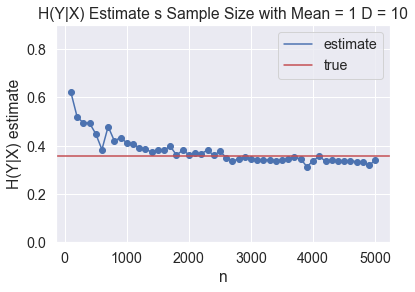
\includegraphics{cond_entropy.png}
    \caption{Empirical demonstration that a variant of decision forests provides a universally consistent estimate of conditional entropy, which can be used as a test statistic for change points.}
    \label{fig:cond_entropy}
\end{figure}

An important aspect of using L2F to estimate conditional entropy and mutual information, is that these statistics can also be used to quantify the ``effect size'', that is, the magnitude of the change.  In fact, many existing definitions of effect size are special cases of MI under certain restrictive parametric settings.  The magnitude of the effect size that we estimate will be important in Section~\ref{sec:combo}.


As a baseline, we will compare this approach to the Oracle approach, which knows when there is a change point.  The metrics would be both concerning the timing of change point detection (how long does it take L2F to detect the change point), and how does the delay impact regret. We will also compare to the parametric approach, which knows the change point time, and the model family, but not the precise distribution, so it must estimate the distribution after each change point. Finally, we hide the change point time from the above parametric approach. Doing so provides a bound on how well one could estimate change points, as compared to our approach. 




\subsection{Continuously Dynamic $P_t$}
\label{sec:smooth}

An even more complicated continual learning setting, and the most general setting, is the case when $P_t$ is itself a continuous stochastic process.  For example, we could assume that $P_t$ follows  first order Markov chain dynamics, meaning that $P_t$ is independent of $P_{t-j}$  for all $j=2,3,...$ when given $P_{t-1}$.  More generally, we can simply assume that the dynamics on $P_t$ are relatively smooth, that is, $|P_t - P_{t-1}| < c$.  Regardless, we must either explicitly or implicitly address the fact that $P_t$ is potentially smoothly changing over time.  

To do so using L2F, we adapt our continual learning L2F described above.  Specifically,~\citet{Cavallanti2007} demonstrated how to track the best hyperplane with a simple budget perceptron.  We will incorporate this technique into each node of our L2F, to enable tracking changes. We will then prove that regardless of the dynamics, the regret of this L2F on any smoothly changing $P_t$, including dynamics produced by reactive environments, will be small.  

The baseline to evaluate this approach would again be the Oracle approach, which knows everything, and the parametric approach, which knows the model family, but does not know the specific parameters. 




\subsection{The Agnostic Setting with Regard to Dynamics of $P$}
\label{sec:combo}


In each of the above settings, we assumed that our L2F had domain knowledge with regard to which of the three settings it was currently facing.  The most general setting, however, is that it is unknown whether $P_t$ is changing, and if so, how it is changing.  Our L2F can also address this setting, although the theoretical guarantees will be weaker, as this setting is dramatically more difficult.  

Specifically, L2F in this context would work as follows.  For each new data point, $z_t$, L2F would continually update, as described in Section~\ref{sec:constant}.  Moreover, L2F would also be checking whether the new sample, and/or the most recent $\tau$ samples are different from the previous epoch's samples using the approach described in Section~\ref{sec:jumps}.  The estimated effect size will be used to weight the amount that the L2F updates the decision boundary under the assumption that things are changing (using Section~\ref{sec:smooth}), versus under the assumption that things are not (using Section~\ref{sec:constant}).  

The baselines here will again be the Oracle, as well as the parametric method with varying degrees of task knowledge. 

\clearpage
\section{Supervised Lifelong Learning}
\label{sec:transfer}

In the above setting, there was a single task, but the data were continually coming, and the distribution of the data was potentially changing.  Here, we consider the case when there are multiple discrete tasks.  Formally, we say that there are two datasets, a source dataset $Z^\mathcal{S}$ and a target dataset $Z^\mathcal{T}$. The source dataset contains $n_s = | Z^\mathcal{S}|$ samples, and the target dataset contains $n_t = |Z^\mathcal{T}|$ samples. In general, these $n_s+n_t$ samples could come from a large number of tasks, but for simplicity, and without loss of generality, we will assume each is associated with a single task. The key that makes a given decision theoretic problem transfer learning, rather than classical learning, is that it is possible that the Bayes decision rule associated with the source task is different from the target task.  The difference could arise due to differences in: the measurement spaces, the distributions, the action spaces, the loss function, or the risk functional, because the Bayes decision rule is a function of each of these things.  The goal of transfer learning it to improve the \emph{rate} of learning on the target task, given the source task. More formally, we assume:
$Z_s \sim F_s$ where $z_s \in \mathcal{Z}_s$ and 
$Z_t \sim F_t$ where $z_t \in \mathcal{Z}_t$. 
The goal is to choose a sequence of learners, $f$, such that the decision rules that they induce result in lower loss than would could achieve without using the source data:
\begin{align}
    \sum_{t=1}^T \ell(\phi_t( \cdot), z_t)    - \inf_{\phi} \sum_{t=1}^T \ell(\phi_t( \cdot, Z^\mathcal{S}), z_t).
\end{align}

A recent publication proposed two mechanisms for using random forests for transfer learning~\cite{Segev2016}, which is quite related to what we originally wrote in our L2F proposal. The two ideas essentially boil down to either (1) updating the structure of given trees, and (2) updating the parameters of the trees (e.g., the features and magnitudes).  The empirical results are impressive, though the theoretical results are limited.  Specifically, whether L2F's constructed in either of these ways achieve universal transfer learning remains an open question.  

Moreover, just because two different tasks are different, does \emph{not} mean that one \emph{should} update the induced decision rules.  Rather, the difference between the two tasks, and the relative amount of new data, dictates whether and how much one should transfer, versus either assuming there has been no difference (which incurs some bias but reduced variance), or ignoring the old data (which incurs no bias but increased variance).  Thus, strong theoretical claims about whether and how much one should transfer remain wide open questions, specifically in the L2F setting.  By virtue of the approach we proposed above to estimate the effect size (in Section~\ref{sec:jumps}), we will be able to ascertain how much mixing to perform, and prove the conditions under which an appropriate degree of mixing is warranted. 

The baselines, therefore, for this task 


\section{Goal Driven Perception}

\section{Latent Task Structure Learning}

\section{Safe Learning}


\end{document}
